\section{Introduction}

    The Higgs Boson sits as the crown jewel of a grand overarching theory of the behavior of the universe,
        known as the Standard Model of Particle Physics.
    While its recent discovery has shed light on many of its key properties,
        there are still many details that are as yet unconfirmed.
    In this chapter, I want to explain what these properties are and how they can be further studied.
    Moreover, I want to justify why the Higgs is so important as to be worth studying in the first place.
    And in order to explain the importance of the Higgs Boson,
        I will need to explain the structure of the Standard Model itself.

    The organization of the following sections will begin with a discussion of the purpose and layout of the Standard Model.
    Following this will be an introduction to the mathematical formalism the Standard Model is based around,
        involving Group Theory, the calculus of variations, and symmetry.
    Here I will introduce the reason for the original postulation of the Higgs, what it is, how it works, and how it fits into the Standard Model.
    Finally, the chapter will conclude with a motivation for further study into the Higgs Boson, and provide a technique to perform such study.
    Additionally, these last sections will introduce the purpose of my particular contribution to the study,
        and lay the groundwork for the techniques used in Chapter \ref{chapter:signal}.

%Matter and Forces
%I need to discuss the elementary particles and their organization before I can really discuss the gauge fields.
%Might as well do it here first and foremost
\section{The Standard Model of Particle Physics}\label{sec:standard_model}
    
    At its core, the Standard Model of Particle Physics is a description of the behavior and interaction of matter.
    Hence, it is necessary to discuss what this matter actually is, first and foremost.
    All known matter can be described as a specific type of elementary particle called a fermion,
        defined by the fact that it contains no discernible substructure and possesses an intrinsic spin of $\hbar/2$.
    These fermions, each with a different mass, are able to interact with each other through three ``fundamental interactions''.
    The three fundamental interactions (more commonly called ``Fundamental Forces'') are known as
        the Electromagnetic, Weak, and Strong interactions (gravity is entirely absent in the Standard Model).
    All the interactions have an associated ``charge'' which can be ascribed to different particles,
        and which govern how strongly that particle can interact with similarly charged particles.
    Indeed, the various fermions are distinct primarily because of the charges they carry.

    \begin{figure}[h!]
        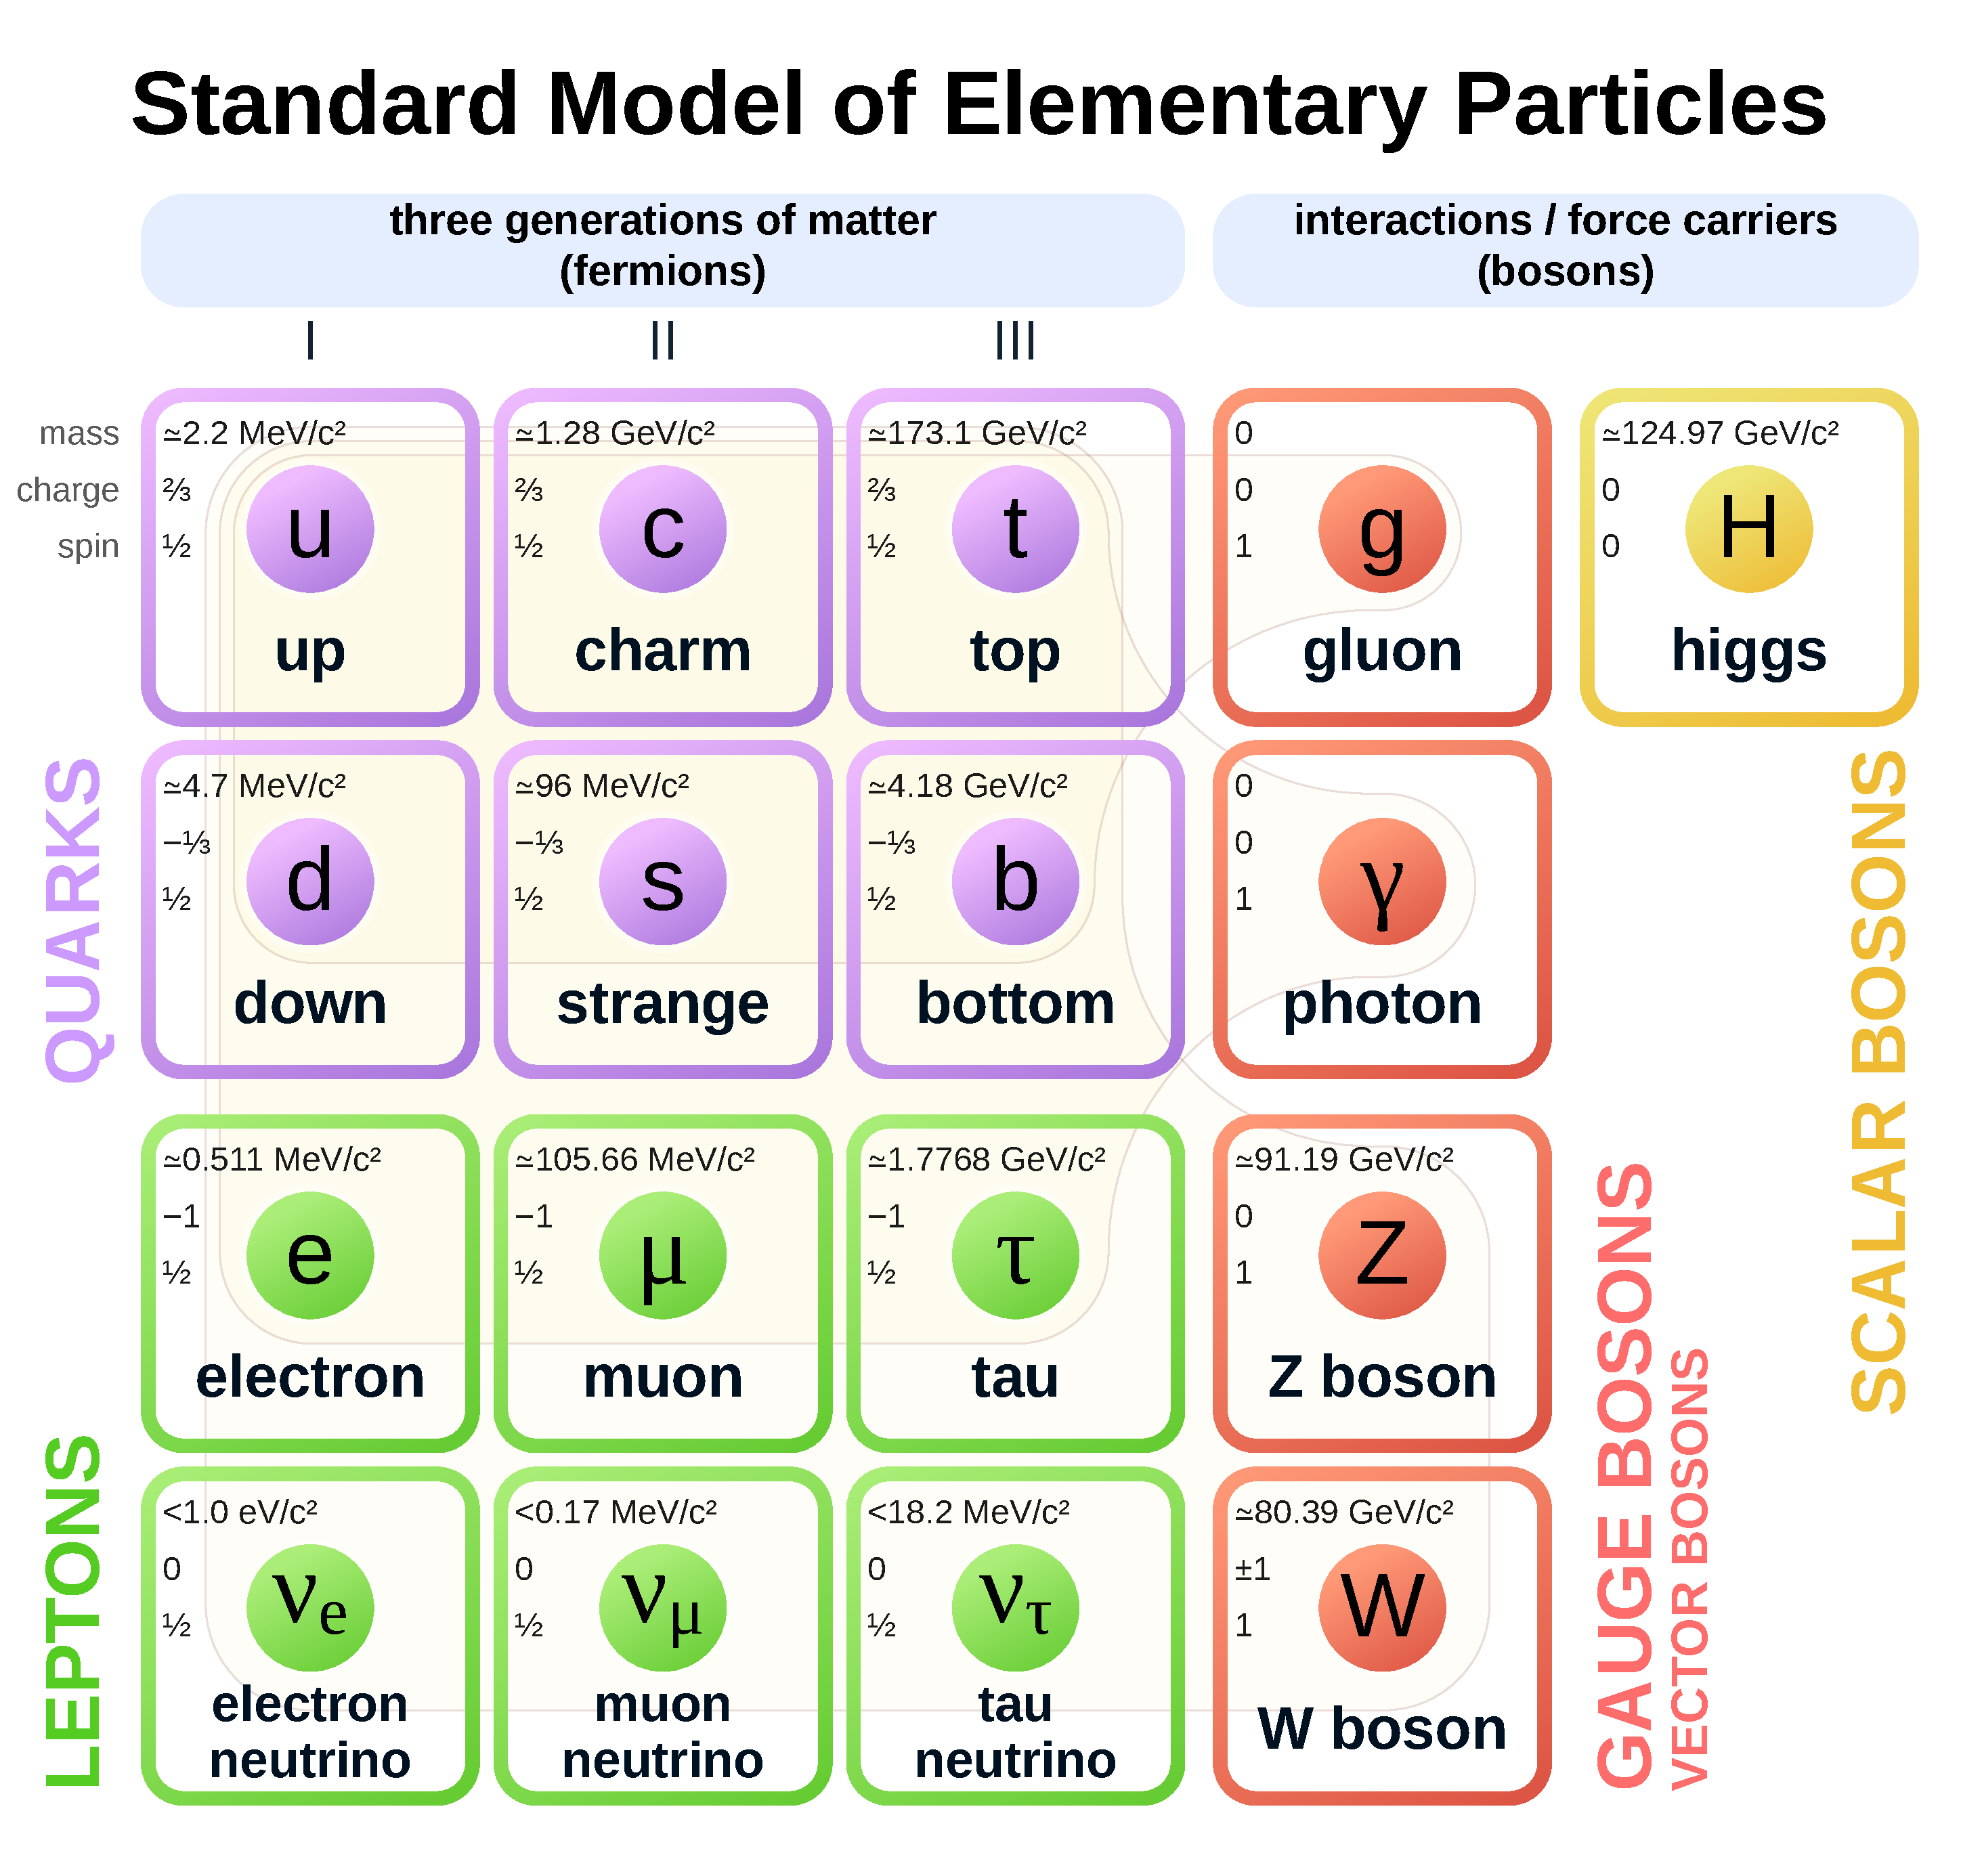
\includegraphics[width=\linewidth,height=\textheight,keepaspectratio]{theory/Standard_Model_of_Elementary_Particles}
        \caption{Table of the particles described by the Standard Model of Particle Physics\cite{wikimedia_sm}
            [FIXME: Hey Steve, I'm using the "online" bibtex style for this reference, but it seems to leave out a ton of information.
                Is that how it's supposed to be? Or do I need to use a different citation category?]}
        \label{fig:sm_particles}
    \end{figure}

    There are twelve distinct elementary fermions (see Figure \ref{fig:sm_particles}),
        which are split evenly into two subgroups, called quarks and leptons.
    Quarks have ``color'' charge associated with the Strong Interaction,
        which leptons lack (and thus cannot interact via the Strong Interaction at all).
    Both classes of particles -- quarks and leptons -- are divided into three ``generations'' of progressively heavier particles.
    Each generation accordingly consists of two quarks and two leptons.
    These pairs, dubbed ``doublets'', behave the same across all generations.
    Among the leptons, every generation contains a doublet of a charged particle (electron, muon, tauon) with EM charge of $\approx −1.6$ coulombs,
        and an uncharged neutrino with no electric charge.
    For quarks, each doublet consists of an up-type quark (up, charm, top) with electromagnetic charge -2/3 that of the electron,
        and a down-type quark (down, strange, bottom) with 1/3 the charge of the electron.
    In addition to the fermions, there is also an entirely separate class of spin 1 particles, called gauge bosons,
        which play a fundamental role in the aforementioned interactions.
    However, an in-depth discussion of these particles will need to wait until Section \ref{sec:gauge_symmetry}.

    The brilliance of the Standard Model lies in how it is able to describe the 
        particles and interactions of nature as consequences of pure mathematical structures.
    Before the mathematical form of particles can be discussed though,
        I must first introduce the mathematics of the setting in which these particles exist:
        the fabric of four-dimensional space-time.


\FloatBarrier
\section{Shape of the Universe: Special Relativity}

    % SR is description of geometry of space-time
    % Encoded in Minkowski metric
    % and utilized via covariant notation
    Special relativity rests on the axiom that the speed of light $c$,
        is an absolute constant that will always appear the same
        \textit{regardless of the speed of an observer}.
    There are many consequences to this, but the most relevant is that
        it produces a description for the geometry of the universe.
    Specifically, it implies that time, rather than a parameter of reality,
        should instead be considered a dimension just as the three spatial dimensions.
    Moreover, a constant speed of light implies that this four-dimensional \textit{space-time} has a particular ``shape,''
        which can be described by how distance within it is measured.
    Just as the familiar three-dimensional (``Euclidean'') distance can be measured with the equation $x^2+y^2+z^2=r^2$,
        four-dimensional space-time (``Minkowskian'') distance is measured as $(ct)^2-x^2-y^2-z^2 = s^2$.
    Basically all classical physics equations assume Euclidean space, and so fall apart in special relativity.
    Physics calculations can be made to abide by special relativity's tenants however,
        by subtly redefining how vector products are evaluated.
    Instead of a vector product defined as
    \begin{equation}
        r^2 = \begin{pmatrix} x & y & z\end{pmatrix} \begin{pmatrix} x \\ y \\ z \end{pmatrix} = \sum\limits_{i=1}^3 x_i x_i
        \quad , \quad \begin{pmatrix}x_1 \\ x_2 \\ x_3 \end{pmatrix} = \begin{pmatrix} x \\ y \\ z \end{pmatrix} 
    \end{equation}

    vector products can be defined with a specific tensor, called the ``metric tensor'' $g$,
        which is inserted between the product's factors and encodes the shape of the particular geometry being used:

    \begin{equation} \begin{split}
        r^2 &= \begin{pmatrix} x & y & z\end{pmatrix}
            \begin{pmatrix}
                1 & 0 & 0 \\
                0 & 1 & 0 \\
                0 & 0 & 1
            \end{pmatrix}
            \begin{pmatrix} x \\ y \\ z \end{pmatrix} \\
        r^2 &= \sum\limits_{i=1}^3 \sum\limits_{j=1}^3 x_i g_i^j x_j
            = \sum\limits_{i=1}^3 x_i x^i
    \end{split} \end{equation}

    In the second line the metric tensor $g_i^j$ has been contracted with $x_j$,
        indicated by the now superscript $x^i$.
    This shorthand convention is called \textit{covariant} notation, and will be used extensively from now on.

    For three-dimensional Euclidean space the metric tensor is just the Identity matrix.
    Four-dimensional space-time is encoded in the Minkowski metric
    \begin{equation}
        \begin{pmatrix}
            1 &  0 &  0 &  0 \\
            0 & -1 &  0 &  0 \\
            0 &  0 & -1 &  0 \\
            0 &  0 &  0 & -1
        \end{pmatrix}
    \end{equation}

    Which permits the appropriate distance equation:

    \begin{equation} \begin{split}
        s^2 &= \begin{pmatrix} ct & x & y & z\end{pmatrix} 
            \begin{pmatrix}
                1 &  0 &  0 &  0 \\
                0 & -1 &  0 &  0 \\
                0 &  0 & -1 &  0 \\
                0 &  0 &  0 & -1
            \end{pmatrix}
            \begin{pmatrix} ct \\ x \\ y \\ z \end{pmatrix} \\
        s^2 &= \sum\limits_{\mu=0}^3 \sum\limits_{\nu=0}^3 x_\mu g_\mu^\nu x_\nu
            \quad , \quad x_0 \equiv ct \\
        s^2 &= x_\mu g_\mu^\nu x_\nu = x_\mu x^\nu
    \end{split} \end{equation}

    Another conventional quirk has been introduced between the final two lines,
        wherein the summations over $\mu$ and $\nu$ are made implicit by the repetition of their indices.
    Known as ``Einstein Summation Notation,'' this convention drastically simplifies equations in Field Theory,
        and will also be used throughout the rest of this thesis.
    With the description of space-time laid out,
        I can now provide a mathematical description for the particles that operate within it.


% QM describes the fundamental resolution limits of the universe
% Resolution limit (uncertainty relation)
% Wave-particle duality and probability states (wave function)
% Operator principle (hermition operators)
\section{Describing Particles: Quantum Field Theory}

    Quantum Field Theory is the mathematical framework the underlies the Standard Model,
        which arises as the confluence of special relativity and quantum mechanics.
    %A comprehensive description of quantum mechanics is less straight-forward than for special relativity,
    %    and its axioms vary depending on the particular formulation used.
    %As such, the following description only seeks to summarize the key aspects of quantum mechanics
    %    directly relevant to the rest of the chapter.
    The most striking feature of quantum mechanics is of course the Heisenberg Uncertainty Principle,
        $\Delta x \Delta p \geq \hbar/2$, which states that there is an absolute lower bound on the
        uncertainty of a particle's position and momentum, defined by the Reduced Planck's Constant $\hbar$.
    Because particles cannot have well defined position and momentum, they can no longer be described as singular objects,
        and instead these properties are described as functions that extend the particle through phase-space.
    The precise form and scope of these functions varies depending on the application and context,
        but in Quantum Field Theory particles are collectively described by a particle \textit{field},
        which exists at all points in space-time, and in which individual particles are merely perturbations of.
    Mathematically, quantum fields are described in the form of linear operators $\varphi(x)$,
        which are functions of all four space-time coordinates.
    These fields operate on \textit{particle states} $\ket{\varphi}$,
        that correspond to the number of a particular type of particle which exists at a given place and time.

    Observable properties of quantum fields (e.g. momentum, spin direction, charge)
        are also represented as operators which operate on the fields.
    The observable quantity of that property is then realized as the eigenvalue of the observable operator.
    Because physically observable quantities must be real-valued,
        quantum mechanics dictates that observable operators must be \textit{Hermitian}
        (the eigenvalues of Hermitian operators are always real)\cite{Griffiths_book}.
    Of these observable operators, perhaps the most fundamental is four-momentum $p^\mu$.
    From the position-representation of the fields,
        four-momentum takes the mathematical form
        %\footnote{
        %    Note that the covariant nature of this definition implies that energy is a positive derivative ($ E/c = p_0 = i \hbar \partial_0 $),
        %        while spatial momentum is a negative derivative ($ p_i = - i \hbar \partial_i, i \in 1,2,3$)
        %}
    \begin{equation}
        p^\mu \equiv i \hbar \frac{\partial}{\partial_\mu} = i \hbar \partial^\mu
    \end{equation}

    Before proceeding to the final description of matter, I want to highlight another notational quirk called ``natural units.''
    A number of physical constants have been mentioned by now, and they are beginning to get cumbersome.
    To address this, an effective (albeit comical) solution is to simply set all of these constants to identically \textit{1}.
    That is, I am setting the speed of light $c$ equal to the reduced Planck's constant $\hbar$,
        equal to the electric charge of the electron, equal to the permittivity of free space $\epsilon_0$,
        and so forth, all equal to 1:
    \begin{equation} c=\hbar=q=\epsilon_0=1 \end{equation}
    There is a potentially profound philosophy to be gleaned from the fact that this can be done at all
        (e.g. for $c$ to literally be unit-less requires that space and time have the \textit{same} units of measurement),
        but I will not delve into such deep implications.
    I (like most textbook authors) am merely taking this to use as a convenient shorthand.
    In this notation, $\{x_0, x_1, x_2, x_3\} \equiv \{t,x,y,z\}$,
        $p^\mu \equiv i \partial^\mu$,
        fermions have spin 1/2,
        electrons have a charge of 1,
        and the famous $E=mc^2$ equation is rendered into the tautological form $E=m$.
    With these conventions and mathematical descriptions in place,
        I can at last express the explicit mathematical form of fermionic matter.

    Fermions are described as manifestations of ``Dirac Fields'', $\psi(x)$,
        which are defined as solutions to an equation of motion known as the Dirac Equation
    \begin{equation} \begin{split}
        (\gamma^\mu p_\mu - m) \psi(x) = 0
        \\ (i\gamma^\mu \partial_\mu - m) \psi(x) = 0
    \end{split} \end{equation}
    The term $\gamma^\mu$ is a vector of matrices, simply called the gamma matrices.
    The derivation and implications of the gamma matrices are a fascinating subject all their own, 
        but for the purposes of this discussion it will suffice to state that
        their primary function is in allowing the 4-vector $p_\mu$ to be added to the scalar $m$.

    Additionally, a peculiar consequence of Quantum Field Theory presents itself in the form of \textit{anti-matter}.
    Anti-matter particle fields correspond to negative-energy\footnote{
            or \textit{time-reversed}, the Feynman-St\"uckelberg interpretation
        } solutions to the Dirac Equation,
        and are represented as
    \begin{equation}
        \psibar(x) \equiv \gamma^0 \psi^\dag(x)
    \end{equation}
    Anti-matter particles are identical to their matter components in every way,
        except that their charges are inverted.

    Describing matter in mathematical form is the first step in building the Standard Model.
    The next step is to do the same with motion.


\section{Generating Motion: Group Theory and Transformations} \label{sec:group_theory}

    An object described by mathematical functions can be ``moved'' using the concept of \textit{transformations}.
    This is accomplished by operating on the function $f$ with a transformation operator $U$ as.
    \begin{equation}
    f \to f' = U f
    \end{equation}

    To see how such an operator works in practice,
        I can start with a simple expression for the position of some object as a function of time, $x(t)$.
    Assuming the object travels with a constant velocity,
        its position can be transformed into a time $\Delta t$ in the future by
    \begin{equation}
    x(t) \to x'(t) = x(t) + v \Delta t
    \end{equation}
    Recognizing that $v$ is just $\frac{d}{dt} x(t)$, this can be rewritten as
    \begin{equation}
    x(t) \to x'(t) = x(t) + \Delta t \frac{d}{dt} x(t) = \left(1+\Delta t \frac{d}{dt}\right) x(t)
    \end{equation}

    This term $\left(1+\Delta t \frac{d}{dt}\right)$ is the classical time-translation operator.
    Notice the assumption of constant velocity though.
    If velocity were not constant, this operator would be invalid,
        except in the specific case for which $\Delta t$ is an infinitesimal $\delta t$.
    \begin{equation}
    x(t) \to x'(t) = \lim_{\delta t \to 0} \left(1+\delta t \frac{d}{dt}\right) x(t)
    \end{equation}

    To produce a more general finite operator I can apply the infinitesimal operator an infinite number of times
    \begin{equation} \begin{split}
    x(t) \to x'(t) &= \lim_{\delta t \to 0} \left(1+\delta t \frac{d}{dt}\right)\left(1+\delta t \frac{d}{dt}\right)\left(1+\delta t \frac{d}{dt}\right)...\ x(t)
    \\x(t) \to x'(t) &= \lim_{N \to \infty} \lim_{\delta t \to 0} \left(1+\delta t \frac{d}{dt}\right)^N x(t)
    \\x(t) \to x'(t) &= \lim_{N \to \infty} \left(1+\frac{\Delta t}{N} \frac{d}{dt}\right)^N x(t)
    \\x(t) \to x'(t) &= e^{\Delta t \frac{d}{dt}} x(t)
    \end{split} \end{equation}

    Where $\Delta t$ is again a finite time transformation,
        and I have compressed the infinite product of terms using the power series expansion of the exponential function.
    In order to use this classical operator in quantum field theory it must of course be Hermitian,
        which requires it to have a factor `$i$' associated with it,
    \begin{equation} \begin{split}
    x(t) \to x'(t) = e^{i\Delta t \frac{d}{dt}} x(t)
    \end{split} \end{equation}

    Returning to Dirac Fields, which are functions of four-position $x_\mu$, this same transformation can be used
         with the minor adjustment of changing the total derivative to a partial derivative in time,
         $\frac{\partial}{\partial t} = \frac{\partial}{\partial x^0} = \partial_0$

    \begin{equation} \begin{split}
    \psi(x) \to \psi'(x) = e^{\Delta x^0 i\partial_0} \psi(x)
    \end{split} \end{equation}

    Meanwhile, the Dirac anti-particle field transforms with a negative sign as
    \begin{equation} \begin{split}
        \psibar(x) \to \psibar'(x) = e^{-\Delta x^0 \partial_0} \psibar(x)
    \end{split} \end{equation}
    
    The time translation operator is but one of a myriad of different transformation operators.
    However, all of the transformation operators used here take a similar form to this, appearing as
    \begin{equation} \begin{split}
        \psi(x) \to \psi'(x) = e^{ q \cdot \mathcal{F}_q } \psi(x)
    \end{split} \end{equation}
    $\mathcal{F}_q$ is the transformation \textit{generator} (e.g.\ $i\partial_0$),
        and $q$ the amount to transform by (e.g.\ $\Delta t$)\footnote{
            Note that the time translation operator from before takes the same form as the quantum mechanical energy operator
                $E = p^0 = i\partial^0$.
            This is no coincidence, as four-momentum is the generator of space-time translations.
         }.

    These transforms fall under a larger realm of mathematics known as Group Theory,
        and are in turn called ``group transformations''.
    The basic definition of a group is a set of elements which can be ``multiplied'' according to some rule,
        and which satisfies the following four conditions\cite{Cheng_book}:
    \begin{itemize}
        \item Closure - the product of any two elements of the group are still in that group;
        \item Associativity - $(a \times b)\times c = a\times(b \times c)$;
        \item Identity - there is some element in the group $I$ for which $I \times a=a$;
        \item and Inversion - every element $a$ has an inverse $a^{-1}$ such that if $b \times a = c$ then $c \times a^{-1} = b$.
    \end{itemize}

    It should be relatively simple to see that time translation operations satisfy each of these.
    Additional classifications for groups are whether a group is discrete or continuous,
        and whether a group is ``Abelian'' (commutative) or ``non-Abelian'' (non-commutative).
    Time translations are continuous (one can translate by an infinitesimally small amount of time),
        and Abelian (the order that the translation are applied does not matter).
    An example of a non-Abelian group would be that of three-dimensional rotations (formally called the $SO(3)$ group),
        as applying rotations in a different order can lead to a different final orientation.

    As a last point regarding Group Theory, is the absolutely crucial idea of \textit{symmetry}.
    If a system can be transformed under a group transformation and remain overall unchanged,
        then that system is said to be invariant, or symmetric, under that group.

    In a very deep sense, Group Theory and symmetry are the driving forces behind the entire Standard Model.
    Not only is the motion of the Standard Model entirely described by Group Theory,
        but as will be seen in the coming sections its interactions are defined by Group Theory,
        and its entire organizational structure ultimately rooted in Group Theory.


\section{Restricting Motion: The Lagrangian and Symmetry}
    
    The Dirac Equation describes the equation of motion of a single field,
        but what is required is a way to describe the interactions of \textit{many} fields.
    For this, the Standard Model makes use of the Principle of Least Action,
        also known as the Lagrangian Formalism\cite{Halzen_book}.
    The idea of the Principle of Least Action is to construct an overall description of all aspects of a system,
        called the Lagrangian, $\Lag$.
    One can then find the ``path'' of this Lagrangian which minimizes the ``Action'', $\mathscr{A}$
    \begin{equation} %TODO: double check this!!
        \mathscr{A} = \int \Lag d^4 x
    \end{equation}

    This minimization is performed using the four-dimensional Euler-Lagrange equations
    \begin{equation}
        \partial_\mu \frac{\partial \Lag}{\partial_\mu \varphi } - \frac{\partial \Lag}{\partial \varphi} = 0
    \end{equation}
    which yields the equations of motion of the interacting particles.

    All of the physics of the Standard Model is inscribed within the Standard Model Lagrangian.
    The construction of this Lagrangian will be the focus of most of the rest of the chapter.
    To begin then, what physics \textit{does} the Lagrangian need to encode?
    Paraphrasing Murray Gell-Mann, ``that which is not forbidden, is \textit{mandatory}\cite{Gell-Mann_mandatory}.''
    That is to say, that any physics which is not expressly prohibited, can and will occur.
    Formulation of the Standard Model Lagrangian must therefore start with an enumeration of restrictions,
        which are given in the form of a series of groups that the Lagrangian must remain symmetric under.
    Specifically, the Lagrangian must remain symmetric under ten transformations,
        collectively referred to as the Poincare Group.
    Four of these transformations correspond to the space-time translations,
        three to spatial rotations, and the remaining three to space-\textit{time} rotations,
        also known as Lorentz Transformations (also known as just changing velocity).

    The Lagrangian of a Dirac field satisfying these symmetries takes the form
    \begin{equation} \label{eq:basic_fermionL}
        \Lag = \psibar (\gamma^\mu p_\mu - m) \psi = i \psibar \gamma^\mu \partial_\mu \psi - m \psibar \psi
    \end{equation}
    As an example of the symmetry now described, I will reuse the time translation operator $e^{i\Delta x^0 \partial_0}$

    \begin{equation} \begin{split}
        \Lag(t) \to \Lag' = \Lag(t+\Delta t) =
            \left( e^{-i\Delta x^0 \partial_0} \psibar \right) (\gamma^\mu p_\mu - m) \left( e^{i\Delta x^0 \partial_0}\psi \right)
        \\  = e^{-i\Delta x^0 \partial_0 + i \Delta x^0 \partial_0} \psibar (\gamma^\mu p_\mu - m) \psi
        \\  = \psibar (\gamma^\mu p_\mu - m) \psi
    \end{split} \end{equation}

    Applying the Euler-Lagrange equations to this equation will separately return the Dirac Equation
        for the fermion and anti-fermion fields, as it should.

    Given that there are many different kinds of fermions, the Lagrangian can be expanded to include all of them
    \begin{equation}
        \Lag = \bar{e} (\gamma^\mu p_\mu - m) e
        + \bar{\mu} (\gamma^\mu p_\mu - m) \mu
        + \bar{\tau} (\gamma^\mu p_\mu - m) \tau
        + \bar{u} (\gamma^\mu p_\mu - m) u
        + ...
    \end{equation}

    Although this equation qualifies as a valid description of the motion of fermions,
        there is a glaring flaw with it: the fields it describes are all completely independent of one another.
    In its current form, the Lagrangian proposes that particles, given some initial momentum,
        will persist along the same trajectory forever, unable to affect or be affected by any other particle.
    Clearly, this is not a satisfactory description of the universe, full of dynamic interactions as it is.
    The resolution to this issue is, counter-intuitively, to enforce yet \textit{more} symmetry requirements.
    In doing so, the various interactions of the Standard Model will be laid bare,
        and the beauty of the theory made apparent.

    %Should I also discuss renormalizability? (Peskin pg 80/101djvu)
    %Basically, all lagrangians must be renormalizable.
    %Renormalizability just means that the lagrangian doesn't explode from the unconstrained nature of virtual particles.
    %So infinite-mass virtual particles should not break a renormalizeable lagrangian.


\section{Generating Interactions: Gauge Symmetry} \label{sec:gauge_symmetry}

    %Describe Global U1
    Allow me to introduce another group, called $U(1)$ (Unitary Rank 1 Group).
    This group corresponds to the phase of a field, and the transformation takes the form
    \begin{equation}
        \psi(x) \to \psi'(x) = e^{i\theta} \psi(x)
    \end{equation}

    %describe global vs local
    As in prior examples, the exponential changes signs for the anti-fermion.
    The generator here is just $i$, the phase shift amount given by the angle $\theta$.
    It is trivial to see that the Lagrangian is invariant under such a group.
    This transformation, along with all the others already described under the Poincare group,
        all fall under the category of \textit{global} transformations.
    A global transformation is one which is applied uniformly across all of space-time.
    There is a different kind of transformation, called a Local or ``Gauge'' transformation.
    Gauge transforms are such that the transformation amount varies \textit{at each point in space-time}.
    A local $U(1)$ transform would then take the form 
    \begin{equation}
        \psi(x) \to \psi'(x) = e^{i\theta(x)} \psi(x)
    \end{equation}
    Noting that the phase-angle $\theta(x)$ is now a function of $x$.

    Demanding that the Lagrangian remain invariant under such a transformation is a much more strict condition,
        one which the current Lagrangian cannot satisfy.
    I want to show how the Lagrangian in its current form breaks when attempting to perform a $U(1)$ gauge transform,
        and how the resolution to this issue demands the existence of a fully dynamic, interacting Lagrangian.

    First, apply the gauge transformation
    \begin{equation} \begin{split}
        \Lag(\theta_0) \to \Lag' = \Lag(\theta_0+\theta(x)) &=
            \left( e^{-i\theta(x)} \psibar \right) (\gamma^\mu p_\mu - m) \left( e^{i\theta(x)}\psi \right)
            \\ &= \left( e^{-i\theta(x)} \psibar \right) i\gamma^\mu \partial_\mu \left( e^{i\theta(x)}\psi \right)
                - \left( e^{-i\theta(x)} \psibar \right) m \left( e^{i\theta(x)}\psi \right)
    \end{split} \end{equation}
    In the mass term, the transform will cancel in the usual fashion.
    The momentum term however will \textit{not} cancel, as the derivative will also affect the position-dependent $\theta(x)$.
    \begin{equation} \begin{split}
        \Lag' &= \left( e^{-i\theta(x)} \psibar \right) i\gamma^\mu \partial_\mu \left( e^{i\theta(x)}\psi \right) - m \psibar(x) \psi(x)
        \\ &= i \left( e^{-i\theta(x)} \psibar \right) \left[
                \left( \gamma^\mu \partial_\mu e^{i\theta(x)} \right) \psi 
                + e^{i\theta(x)} \left( \gamma^\mu \partial_\mu \psi \right)
            \right] - m \psibar(x) \psi(x)
        \\ &= i \left( e^{-i\theta(x)} \psibar \right)
                \left( \gamma^\mu \partial_\mu e^{i\theta(x)} \right) \psi 
            + i \psibar \gamma^\mu \partial_\mu \psi
            - m \psibar(x) \psi(x)
        \\ &= - \psibar \left( \gamma^\mu \partial_\mu\theta(x) \right) \psi 
            + \psibar ( \gamma^\mu p_\mu - m ) \psi
    \end{split} \end{equation}

    %Show how to fix lagrangian
    Under a local $U(1)$ transform, $\Lag$ is clearly not invariant,
        due to the additional $\gamma^\mu \partial_\mu\theta(x)$ term.
    In order to enforce gauge symmetry, a subtle but profound adjustment must be made to the Lagrangian.
    This adjustment will take the form of a modification to the derivative,
        replacing the standard derivative with a \textit{covariant} derivative,
    \begin{equation}
        \partial_\mu \to D_\mu \equiv \partial_\mu + i \emc A_\mu(x)
    \end{equation}
    where $\emc$ is a constant and the new function $A_\mu(x)$ is formulated such that it transforms under a $U(1)$ gauge rotation as
    \begin{equation}
        A_\mu(x) \to A'_\mu(x) = A_\mu(x) - \frac{1}{\emc} \partial_\mu \theta(x)
    \end{equation}

    With this additional term, the Lagrangian becomes
    \begin{equation} \begin{split}
    \Lag = \psibar (i\gamma^\mu D_\mu - m) \psi
        = \psibar \left[i\gamma^\mu(\partial_\mu + i \emc A_\mu) - m\right] \psi
    \end{split} \end{equation}
    and the specific transformation property of $A$ renders the entire equation invariant under a gauge transform
    \begin{equation} \begin{split}
    \Lag(\theta_0) \to \Lag' &= \Lag(\theta_0+\theta(x))
        \\&= \left( e^{-i\theta(x)} \psibar \right) 
        \left[i\gamma^\mu \left(\partial_\mu 
            + i \emc \left[A_\mu - \frac{1}{\emc} \partial_\mu \theta(x)\right] \right) 
            - m\right]
        \left( e^{i\theta(x)}\psi \right)
        \\&= \psibar \left[i\gamma^\mu(\partial_\mu + i \emc A_\mu) - m\right] \psi
    \end{split} \end{equation}

    % Introduce photon field and show newly produced interaction
    % See Peskin pg484 (djvu 505) for derivation of kinetic term
    % See also https://physics.stackexchange.com/questions/131097/gauge-field-tensor-from-wilson-loop
    Through a much more sophisticated derivation (which will not be demonstrated here),
        it can also be shown that this new covariant derivative causes the Action to acquire an additional term 
        related to the commutator of the covariant derivative, $[D_\mu, D_\nu] \equiv D_\mu D_\nu - D_\nu D_\mu$.
    Defining a tensor $F_{\mu\nu}$ as $i\emc F_{\mu\nu} = [D_\mu, D_\nu]$,
        the additional required term takes the form $-\frac{1}{4}F^{\mu\nu}F_{\mu\nu}$.
    The final expression for the $U(1)$ gauge invariant fermion Lagrangian now appears as
    \begin{equation} \label{eq:qedL} \begin{split}
        \Lag &= \psibar (i\gamma^\mu D_\mu - m) \psi - \frac{1}{4}(F_{\mu\nu})^2
        \\&= i \psibar \gamma^\mu \partial_\mu \psi
            - m \psibar \psi
            + i \emc \psibar \gamma^\mu A_\mu \psi
            - \frac{1}{4}F_{\mu\nu}F^{\mu\nu}
    \end{split} \end{equation}

    Of extraordinary note is that the last term of $\Lag$ is completely independent of the Dirac field $\psi$.
    The true nature of $A$ is thus revealed, not as just a mere correction factor,
        but as a massless field all its own.
    Indeed, $A(x)$ corresponds to the photon field, $\emc$ to the electric charge,
        and the term $-\frac{1}{4}(F_{\mu\nu})^2$ to the kinetic energy of the photon.
    Furthermore, the three-field term $i \emc \psibar \gamma^\mu A_\mu \psi$
        allows the Dirac field to interact directly with the photon field,
        and through the photon field to interact indirectly with \textit{other} Dirac fields.
    Far from the static situation described by Equation \ref{eq:basic_fermionL},
        the new Lagrangian permits a wide range of dynamic interactions between particles.
    In fact, using the Euler-Lagrange equations on Equation \ref{eq:qedL}
        will now reproduce the Lorentz Force Law as the equation of motion for the Dirac fields,
        and Maxwell's Equations as the equation of motion for the photon.

    % Introduce SU(2) and SU(3)
    All of this complexity arose from the simple imposition of the $U(1)$ gauge symmetry upon the fermion Lagrangian.
    The full extent of interaction in the Standard Model can be realized by imposing then two more gauge group symmetries:
        $SU(2)$, and $SU(3)$.
    Both of these groups behave in a similar manner to $U(1)$, with the transformations taking the forms
    \begin{equation} \begin{split}
        SU(2)&: e^{i \alpha^a(x) \sigma^a / 2}, a=\{1,2,3\}
        \\SU(3)&: e^{i \xi^b(x) \mathscr{F}^b / 2}, b=\{1,2, ..., 8\}
    \end{split} \end{equation}
    where $\sigma^a$ corresponds to the three, $2 \times 2$ Pauli Matrices
    \begin{equation}
        \sigma^1 = \begin{pmatrix} 0 & 1 \\ 1 & 0 \end{pmatrix} \quad
        \sigma^2 = \begin{pmatrix} 0 & -i \\ i & 0 \end{pmatrix} \quad
        \sigma^3 = \begin{pmatrix} 1 & 0 \\ 0 & -1 \end{pmatrix}
    \end{equation}
    and $\mathscr{F}^b$ corresponds to the eight $3 \times 3$ Gell-Mann matrices of $SU(3)$
        (which will not be explicitly written out).

    While $U(1)$ acted as a one-dimensional rotation of a single complex angle $\theta$,
        $SU(2)$ performs three orthogonal rotations $\alpha^a$ through a three-dimensional complex space,
        and $SU(3)$ performs rotations through an eight-dimensional complex space.
    Because $SU(2)$ operates through the $2 \times 2$ Pauli Matrices, it must operate on the fermions in doublets
        (recall Section \ref{sec:standard_model}).
    \begin{equation}
        \minimatrix{u_L \\ d_L} \to e^{i \alpha^a \sigma^a / 2} \minimatrix{u_L \\ d_L}
    \end{equation}

    Similarly, the triplet nature of $SU(3)$ necessitates that the group operate on all three generations of fermions at once
    \begin{equation}
        \minimatrix{u\\c\\t} \to e^{i \xi^b \mathscr{F}^b / 2} \minimatrix{u\\c\\t}
    \end{equation}

    Neither group operates uniformly across the fermions though.
    $SU(2)$ acts only on the ``left-handed'' chiral state of the fermions (denoted by the subscript L),
        and $SU(3)$ acts only on the quarks, having a charge of zero for all leptons.

    The behavior of these Gauge Groups established, the natural assumption is that the three gauge fields
        $U(1)$, $SU(2)$, and $SU(3)$ correspond to the three fundamental interactions,
        Electromagnetic, Weak, and Strong.
    This would serve to complete a theory of the universe based entirely on the geometric principle of symmetry.
    The electromagnetic interaction and its photons have already been revealed as the manifestation of the $U(1)$ group. 
    Likewise, $SU(3)$ assuredly does correspond to the strong interaction, its gauge fields manifested as the Gluons.
    All of this breaks down however with $SU(2)$, which does \textbf{not} directly correspond to the W and Z bosons.

    The problem is that the W and Z fields have mass.
    Gauge fields in this formalism \textit{cannot} have mass.
    A brief check will confirm that a Lagrangian mass term such as $m_Z^2 (Z^0)^2$
        will not remain invariant under the gauge field's own transformation.
    By all rights, the experimental measurement of the W and Z masses should have
        ended the idea of gauge symmetry as a principle of nature altogether.
    Instead, a theory was proposed which would allow gauge symmetry to persist,
        but only under the condition that an entirely new field, unlike any previously observed, must exist.
    Not only did this theory resolve the origin of the W and Z masses;
        it predicted -- nearly a half-century in advance of its discovery --
        the existence of the scalar particle now known as the Higgs Boson.
    \cite{Osborn_notes}
    \cite{Peskin_book}
    \cite{Halzen_book}

